\documentclass[11pt]{article}

\usepackage{amsmath, amssymb}
\usepackage{graphicx}
\usepackage{xcolor}
\usepackage{booktabs}
\usepackage{geometry}
\usepackage{booktabs,longtable,array}
\usepackage[hidelinks]{hyperref}

\geometry{margin=1in}

\title{Modelling mass TB and TBI screening in South Tarawa (Kiribati) --- Technical appendix}
\date{}
\author{Romain Ragonnet}

\begin{document}

\maketitle

\tableofcontents
\clearpage

%%%%%%%%%%%%%%%%%%%%%%%%%%%%%%%%%%%%%%%%%%%%%%%%%%%%%%%%%%%%
\section{Overview of the Model and Analysis}

We developed a deterministic, age-structured compartmental model of \textit{Mycobacterium tuberculosis} (M.tb) transmission, infection, disease, detection, treatment, and prevention. The model uses discrete age groups and continuous time, and is formulated as a system of ordinary differential equations (ODEs).

\paragraph{Compartment notation (per age group).}
We denote the following compartments:
\begin{itemize}
    \item \(\mathbf{S}\): M.tb-\emph{na\"ive} (never infected).
    \item \(\mathbf{E}\): Incipient infection (post-infection with risk of disease progression).
    \item \(\mathbf{C}\): Contained infection (immune control without sterilisation - no immediate disease progression risk).
    \item \(\mathbf{X}\): Cleared infection (post infection clearance - spontaneous or TPT-induced).
    \item \(\mathbf{D_{SL}}\): Active TB, \underline{S}ubclinical, \underline{L}ow infectiousness.
    \item \(\mathbf{D_{CL}}\): Active TB, \underline{C}linical, \underline{L}ow infectiousness.
    \item \(\mathbf{D_{SH}}\): Active TB, \underline{S}ubclinical, \underline{H}igh infectiousness.
    \item \(\mathbf{D_{CH}}\): Active TB, \underline{C}linical, \underline{H}igh infectiousness.
    \item \(\mathbf{T}\): On TB treatment.
    \item \(\mathbf{R}\): Recovered (post self-recovery or treatment).
\end{itemize}

\noindent We use the term ``M.tb na\"ive'' rather than the commonly used ``Susceptible'' to describe individuals who have never been infected with M.tb, because several non-na\"ive compartments remain (partially) susceptible to reinfection.

\paragraph{Model overview.}
Non-disease \emph{M.~tuberculosis} infection is modelled through two stages: incipient (\(E\)) and contained (\(C\)). 
The contained stage represents a state in which the infection is controlled by the immune system, with no immediate risk of progression to active disease. 
Breakdown of containment reflects loss of immune control, returning individuals to the incipient stage (\(E\)) with a renewed risk of disease progression. 
Containment can also result in complete clearance of infection, represented by state \(X\).

Progression from \(E\) results in subclinical active disease (more or less infectious) that may gain/lose infectiousness and progress/regress between clinical and subclinical states. More details about the disease categorisation and transitions are provided in Section~\ref{sec:tb_disease}. 
Only \emph{clinical} forms of disease are detected through passive case finding; while active screening may potentially detect any form of TB. Screening programmes add time-limited detection flows for both TB disease and non-disease M. tb infection states (Section~\ref{sec:screening}).

Age-specific demography and mixing are implemented explicitly to capture the effects of population structure and contact patterns on transmission dynamics (Sections~\ref{sec:demog}--\ref{sec:mixing-matrix}).

\paragraph{Model structure.}
\begin{figure}[!ht]
\centering
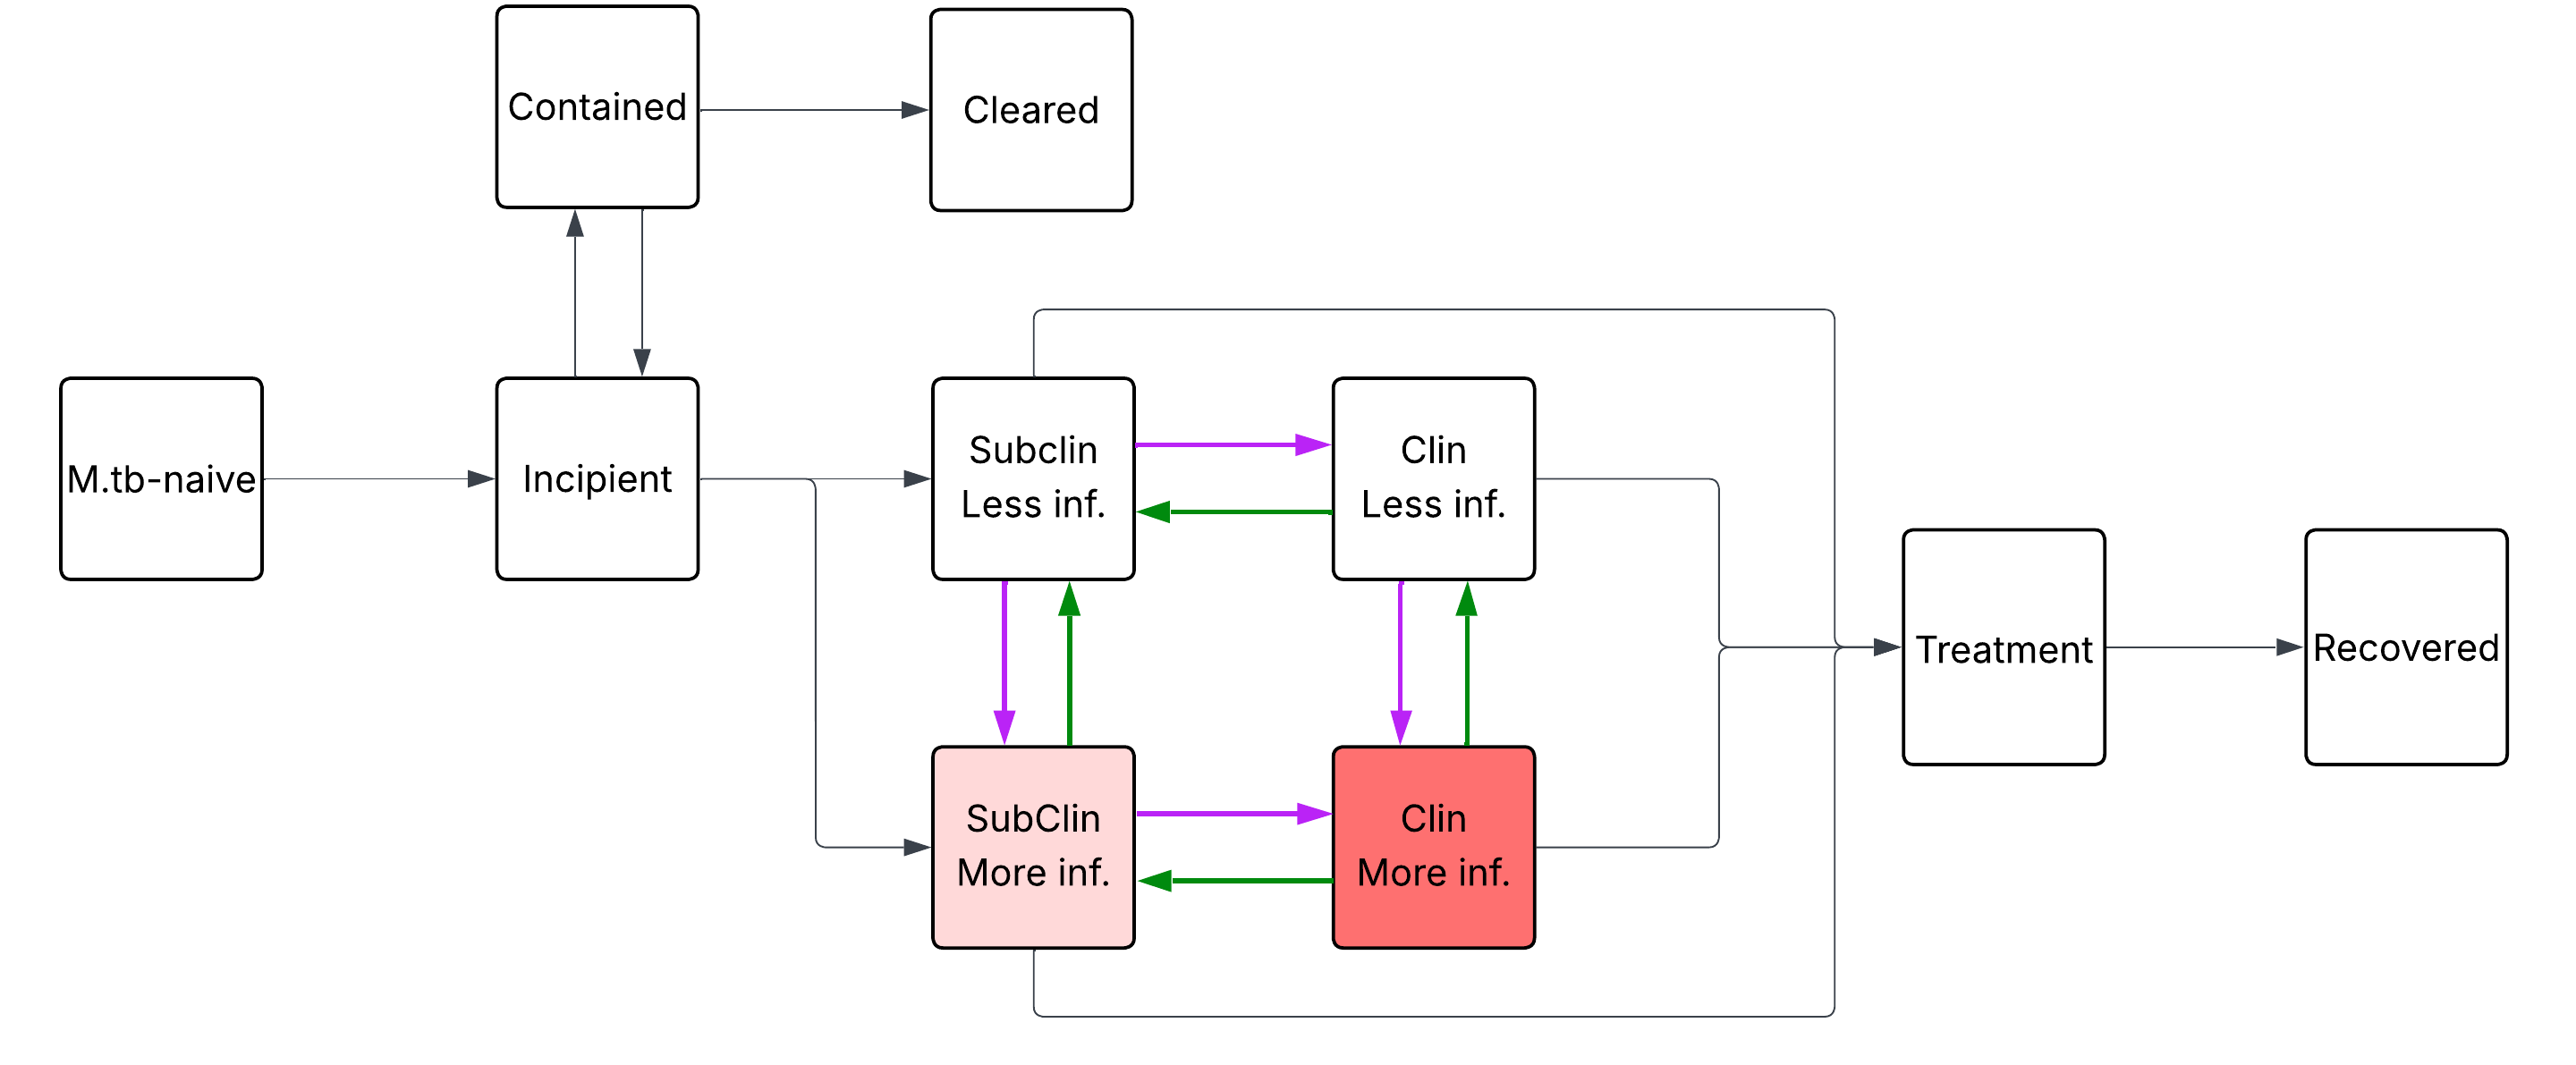
\includegraphics[width=0.95\textwidth]{figures/tb_model.png}
\caption{Schematic of model compartments and transitions.}
\label{fig:model-structure}
\end{figure}

\paragraph{Parameter treatment in calibration.}
Parameters with specified prior distributions are estimated in the Bayesian calibration while those without priors are fixed. 
Estimated classes include core transmission (baseline transmission rate and population-scaling exponent), social mixing (background mixing level, age assortativity spread, and parent–child mixing strength), selected early-infection and disease-transition rates (clearance, immunity breakdown, clinical progression, gain of infectiousness), the passive-detection scale-up profile, and a subset of diagnostic sensitivities. 

\paragraph{Model use in analysis.}
The model is used in two stages: (i) to reconstruct the historical epidemic trajectory by calibrating uncertain parameters to epidemiological and intervention data; and (ii) to project forward under alternative intervention scenarios (screening and preventive treatment). Parameter estimation is performed in a Bayesian framework with Differential Evolution Metropolis algorithm (DEMetropolisZ); posterior samples are propagated to quantify uncertainty in projected outcomes.

%%%%%%%%%%%%%%%%%%%%%%%%%%%%%%%%%%%%%%%%%%%%%%%%%%%%%%%%%%%%
\section{Software and Code}

The model is implemented in Python using \texttt{summer2}, enabling symbolic specification and efficient numerical ODE generation. Computations are accelerated via \texttt{jax} just-in-time compilation, which lowers the ODE system to optimised machine code after first execution; subsequent simulations require \(\sim\)200\,ms each, enabling large-scale Bayesian calibration.

All model code, calibration routines, analysis scripts, and interactive notebooks are available at \url{https://github.com/monash-emu/tb_hierarchical}.

The repository includes instructions for installation and reproduction of results (\textcolor{red}{Need to work on this}). The project environment is managed using \texttt{pixi} for reproducible dependency management and straightforward installation.

%%%%%%%%%%%%%%%%%%%%%%%%%%%%%%%%%%%%%%%%%%%%%%%%%%%%%%%%%%%%
\section{Demographics}
\label{sec:demog}

Each age and disease state in the model is subject to the appropriate all‑cause and TB‑specific mortality rates. Non-TB deaths are calculated using time-variant and age‑specific mortality rates, and births are injected into the youngest M.tb-naïve compartment to reproduce the observed population size over time.
This approach allows the model to match observed population trajectories while maintaining internal demographic dynamics. Age‑specific mortality rates and population size over time are taken from the United Nations World Population Prospects (WPP) data. 
We implement ageing as first-order transitions between adjacent age groups, with rates calculated as the inverse of the age group's span and applied to all age strata except the oldest one.
%%%%%%%%%%%%%%%%%%%%%%%%%%%%%%%%%%%%%%%%%%%%%%%%%%%%%%%%%%%%
\section{Natural History of Infection and Disease}
We represent early TB infection dynamics using two non-disease states: an \emph{incipient} state (E) and a \emph{contained} state (C). Individuals newly infected with \emph{M. tb} enter E, where infection is unstable and at risk of progression. From E, they may either progress to subclinical active TB or undergo immune-mediated containment, moving to C. Contained infection may subsequently clear entirely to X (uninfected/cleared) or experience immunological failure, returning to the incipient state E.
Active TB is stratified by both clinical presentation (subclinical vs. clinical) and infectiousness (low vs. high), yielding four disease compartments: $D_{SL}, D_{CL}, D_{SH}, D_{CH}$. Individuals with subclinical disease may progress to clinical disease, and clinical disease may regress to subclinical; similarly, infectiousness may increase (low $\to$ high) or decrease (high $\to$ low).
However, transitions are restricted to a single dimension at a time. Individuals may change clinical status (subclinical $\leftrightarrow$ clinical) or infectiousness (low $\leftrightarrow$ high), but simultaneous transitions in both dimensions are not allowed. 
Self-recovery is allowed only from subclinical states, with recovered individuals entering $R$. In contrast, TB-induced mortality rates are only applied to the clinical states.
Treatment is available for all active states, with successful treatment leading to recovery ($R$) and unsuccessful treatment resulting in relapse to subclinical low infectiousness ($D_{SL}$) or death.

\paragraph{Early infection.}
Progression from \(E\) is age-specific (three categories: $<5$, 5--14, 15+) and partitioned into low vs high infectiousness at first presentation. Containment rates are also age-specific. Clearance and immune breakdown are age-invariant.

\paragraph{Clinical and infectiousness transitions.}
\label{sec:tb_disease}
Movements between subclinical and clinical states and between low and high infectiousness govern within-disease dynamics. Clinical progression and gain of infectiousness are estimated; clinical regression and loss of infectiousness are fixed.

\paragraph{Infectiousness weighting.}
Let \(\sigma_S\) denote the relative infectiousness of subclinical vs clinical disease, and \(\sigma_L\) the relative infectiousness of low vs high. Define the active-disease index set
\[
\mathcal{K}=\{SL,CL,SH,CH\},
\]
with relative infectiousness weights \(w_k\) given by \(w_{CH}=1\), \(w_{CL}=\sigma_L\), \(w_{SH}=\sigma_S\), \(w_{SL}=\sigma_S\sigma_L\). Children under 15 years contribute zero infectiousness, implemented by setting \(w_k=0\) in those age groups.

%%%%%%%%%%%%%%%%%%%%%%%%%%%%%%%%%%%%%%%%%%%%%%%%%%%%%%%%%%%%
\subsection{Generalised Transmission and Infectiousness Weights}

We interpolate between frequency- and density-dependent transmission using the exponent \(\kappa\in[0,1]\) applied to the contacted population size. The force of infection for age group \(i\) is
\[
\lambda_i(t)
=
\beta_0\, N_{\mathrm{ref}}^{\,\kappa}
\sum_{j}
\tilde{C}_{ij}(t)\;
\frac{I^{\mathrm{eff}}_j(t)}{N_j(t)^{\kappa}},
\]
where \(\tilde{C}(t)\) is the spectral-radius-normalised age-mixing matrix (Section~\ref{sec:mixing-matrix}).  Here \(N_{\mathrm{ref}}\) denotes the total population in year 2020 and is included purely as a scaling constant for more efficient calibration. This rescaling stabilises the magnitude of the transmission coefficient \(\beta_0\) across different values of \(\kappa\), preventing its calibrated value from varying by orders of magnitude as the dependence on population size changes.
The effective infectious pool in age group \(j\) is expressed as an indexed sum:
\[
I^{\mathrm{eff}}_j(t) =
\sum_{k\in\mathcal{K}} w_k\, D_{k,j}(t).
\]
Individuals $<15$\,y contribute zero infectiousness (weights set to zero in those age groups).

%%%%%%%%%%%%%%%%%%%%%%%%%%%%%%%%%%%%%%%%%%%%%%%%%%%%%%%%%%%%
\subsection{Reinfection Pathways}

Reinfection is permitted from \(C\), \(X\), and \(R\) with relative susceptibilities \(\rho_C\) (contained) and \(\rho_X=\rho_R\) (cleared and recovered), and a child susceptibility modifier \(\sigma^{\text{child}}\) applied when infection arises from \(S\) in $<15$\,y groups.
This adjustment captures the effect of BCG vaccination, which is typically administered in infancy and provides protection against infection for several years.

%%%%%%%%%%%%%%%%%%%%%%%%%%%%%%%%%%%%%%%%%%%%%%%%%%%%%%%%%%%%
\section{Age Stratification and Mixing}

%%%%%%%%%%%%%%%%%%%%%%%%%%%%%%%%%%%%%%%%%%%%%%%%%%%%%%%%%%%%
\subsection{Ageing and Age-Specific Adjustments}

\paragraph{Age groups.}
The population is stratified into \(G = 8\) age groups with lower bounds
\[
\mathcal{A} = \{0, 3, 5, 10, 15, 18, 40, 65\}.
\]
The final group is open-ended (65+).

\paragraph{Ageing and adjustments.}
Ageing is implemented as first-order transitions between adjacent age groups. Several age-specific adjustments and interventions are applied in the model (see previous sections for details):

\begin{itemize}
\item Age-specific early infection rates using three categories: \(<5\) years, 5--14 years, and 15+ years.
\item Reduced susceptibility to infection from \(S\) in individuals aged \(<15\) years to reflect BCG effect.
\item Infectiousness set to zero for individuals aged \(<15\) years.
\item Age-specific background mortality.
\item Age-specific screening interventions.
\end{itemize}

%%%%%%%%%%%%%%%%%%%%%%%%%%%%%%%%%%%%%%%%%%%%%%%%%%%%%%%%%%%%
\subsection{Age-Mixing Matrix}
\label{sec:mixing-matrix}

\paragraph{Notation and data sources.}
Let \(i,j \in \{1,\dots,G\}\) index age groups and \([a_i,b_i]\) denote the single ages in group \(i\). Calendar time is \(t\) (years). 
We use UN World Population Prospects data to inform age-specific population sizes (1950--2100) and age-specific fertility rates (1950--2023). For modelled years outside data ranges, quantities are clamped to the nearest available year.
\paragraph{Overview.}
At time \(t\), we construct an age-specific contact matrix
\[
\mathbf{C}(t) = \big(C_{ij}(t)\big)_{i,j=1}^G,
\]
where \(C_{ij}(t)\) is the per-capita rate at which age group \(i\) contacts age group \(j\). Construction proceeds by:
(1) building a symmetric per-pair intensity matrix \(\mathbf{S}(t)\);
(2) scaling columns by the contacted group size;
(3) normalising by the spectral radius.
We combine three components: uniform background mixing, assortative age mixing, and parent–child mixing. Three scalar parameters govern these components (background level, assortativity spread, and parent–child mixing strength) and are estimated.

\paragraph{Population weights within age groups.}
To allow non-uniform single-age distributions within groups, let \(N(a,t)\) be the population at age \(a\) and time \(t\). For group \(i\),
\[
w_i(a,t) = \frac{N(a,t)}{\sum_{a' \in [a_i,b_i]} N(a',t)},\qquad
\sum_{a \in [a_i,b_i]} w_i(a,t)=1.
\]

\paragraph{Symmetric per-pair intensity.}
For each \(i,j\),
\[
S_{ij}(t) = b + S^{\mathrm{assort}}_{ij}(t) + \kappa_{\mathrm{pc}}\, S^{\mathrm{pc}}_{ij}(t),
\quad S_{ij}(t)=S_{ji}(t),
\]
where \(b\) is the background level, \(S^{\mathrm{assort}}\) is an exponential kernel with spread \(a\), and \(S^{\mathrm{pc}}\) encodes parent–child contacts from fertility patterns.

\emph{Assortative age mixing.}
\[
S^{\mathrm{assort}}_{ij}(t)
=
\sum_{a \in [a_i,b_i]}
\sum_{c \in [a_j,b_j]}
w_i(a,t)\, w_j(c,t)\,
\frac{1}{a}
\exp\!\left(-\frac{|a-c|}{a}\right).
\]

\emph{Parent–child mixing.}
Let \(p_{\mathrm{pc}}(\Delta, y)\) be the probability of a parent–child age gap \(\Delta\) for a child born in year \(y\). With \(a_{\mathrm{child}}=\min(a,c)\) and birth year \(t-a_{\mathrm{child}}\),
\[
S^{\mathrm{pc}}_{ij}(t)
=
\sum_{a \in [a_i,b_i]}
\sum_{c \in [a_j,b_j]}
w_i(a,t)\, w_j(c,t)\,
p_{\mathrm{pc}}\!\left(|a-c|,\; t - a_{\mathrm{child}}\right).
\]

\paragraph{Population scaling and asymmetry.}
The per-pair matrix becomes an asymmetric WAIFW matrix by column scaling with the contacted group size:
\[
C_{ij}(t) = S_{ij}(t)\, N_j(t).
\]

\paragraph{Normalisation.}
Let \(\rho(t)\) be the spectral radius of \(\mathbf{C}(t)\). We use the normalised matrix
\[
\tilde{\mathbf{C}}(t) = \frac{\mathbf{C}(t)}{\rho(t)}.
\]

%%%%%%%%%%%%%%%%%%%%%%%%%%%%%%%%%%%%%%%%%%%%%%%%%%%%%%%%%%%%
\section{TB Detection, Treatment and Screening}
\label{sec:screening}

\subsection{Detection}

\paragraph{Passive detection.}
Passive case finding applies \emph{only to clinical disease}. Subclinical disease is not detected passively. Denote the time-varying passive detection profile by \(\delta(t)\), which follows a smooth hyperbolic-tangent scale-up from an earlier (lower) level to a recent level:
\[
\delta(t)
=
\delta_{\mathrm{rec}}
\Bigg[
\phi
+
(1-\phi)\,
\Bigg(
\frac{\tanh\!\big(\sigma\, (t - t^\ast)\big)}{2}
+
\frac{1}{2}
\Bigg)
\Bigg].
\]
Here, \(\delta_{\mathrm{rec}}\) is the recent detection level, \(\phi\in(0,1]\) is the past-to-recent ratio, \(\sigma>0\) controls steepness, and \(t^\ast\) is the inflection time.

Figure~\ref{detect} illustrates an example profile for 
$\delta_{\mathrm{rec}} = 0.7$, $\phi = 0.5$, $\sigma = 0.15$ and $t^\ast = 2005$.
\begin{figure}[!ht]
\centering
\includegraphics[width=0.6\textwidth]{figures/pdetection_profile.png}
\caption{Example time-varying passive detection profile for clinical TB disease.}   
\label{detect}
\end{figure}

\subsection{Screening programmes}

We consider a set of time-limited screening interventions implemented over the year 2026. 
Each screening programme is defined by a screening algorithm, a target population (by age), and a coverage level. 
Five coverage levels are explored: low (55\%), medium (65\%), high (75\%), very high (85\%), and maximum (95\%). These correspond to the proportion of the target population reached over the duration of the campaign.

For each programme, the total coverage is translated into a constant per-capita screening rate over the intervention period. Specifically, if \(c\) denotes the target coverage (expressed as a proportion) and \(\Delta t\) the duration of the campaign, 
the screening rate is defined as \(-\frac{\log(1 - c)}{\Delta t}\).

This ensures that, under a constant hazard assumption, a proportion \(c\) of the target population is screened over the intervention period. The screening rate is implemented as a time-varying function that is zero outside the intervention window and constant during the campaign.

Screening interventions may act on TB infection or active TB disease states. For each screening algorithm, screened individuals have a probability of being correctly identified defined by the sensitivity of the relevant algorithm for that compartment. 
For TB screening, positively screened individuals are moved to the treatment compartment (\(T\)). 
For TPT, only a fraction of the positively screened individuals transition to the cleared compartment (\(X\)) based on the probability of successful TPT completion.

\paragraph{Screening algorithms.}

We consider the following screening tools which all have state-specific sensitivities, some of which are estimated in the calibration while others are fixed based on literature or observations during the PEARL study implementation.

\begin{itemize}
    \item \textbf{Symptom screening (SSx)}   
    \item \textbf{Chest X-ray (CXR)}    
    \item \textbf{Pluslife tongue swab (PLTS)} 
    \item \textbf{Xpert}
    \item \textbf{Tuberculin skin test (TST)} 
\end{itemize}

\paragraph{Age targeting.}
Screening programmes are targeted to specific age groups by applying multiplicative coverage adjustments during model age stratification. Age groups not targeted by a given programme have zero screening rate.

\paragraph{Scenario structure.}
We consider 25 scenarios grouped into five sets:

\begin{itemize}
    \item \textbf{Scenarios 1--5 (PEARL):} PEARL algorithm as implemented during the first phase of the PEARL study. Individuals aged 10 years and above receive CXR combined with Xpert testing (in 35\% of individuals), while children aged 3--9 years receive symptom screening and TST is applied to individuals aged 3 years and above.
    
    \item \textbf{Scenarios 6--10 (CXR-TST):} Xpert is removed; CXR is used for individuals aged 10 years and above, with symptom screening for ages 3--9 years and TST for ages 3 years and above.
    
    \item \textbf{Scenarios 11--15 (CXR-TST, 10+ only):} Screening is restricted to individuals aged 10 years and above, using CXR and TST; no screening is performed in children under 10 years.
    
    \item \textbf{Scenarios 16--20 (CXR only, 10+):} Screening is further simplified to CXR only for individuals aged 10 years and above.
    
    \item \textbf{Scenarios 21--25 (CXR-PLTS-TST):} Tongue swab testing (PLTS) replaces Xpert; CXR and PLTS are used for individuals aged 10 years and above, with symptom screening for ages 3--9 years and TST for ages 3 years and above.
\end{itemize}

Within each group, the five coverage levels are applied, resulting in a total of 25 scenarios. This framework allows us to assess the incremental impact of alternative diagnostic strategies, the removal of specific tools (e.g.\ Xpert or TST), and the effect of restricting screening to older age groups.

\subsection{Treatment outcomes}
During treatment, individuals may experience three mutually exclusive outcomes: successful recovery, relapse, or death. Recovery occurs at a rate depending on the time-varying treatment success rate:
\[
\text{Recovery: } \quad \text{rate} = \frac{\text{TSR}(t)}{\tau},
\]
where \(\text{TSR}(t)\) denotes the proportion of successful treatments at time \(t\), and \(\tau\) is the average treatment duration.  

Age-specific relapse and treatment-death rates are calculated to account for both background mortality and the fixed proportion of treatment episodes that result in negative outcomes. Let \(\mu_i\) be the natural mortality rate for age group \(i\). The fixed fraction of negative outcomes resulting in death is denoted \(f_\text{neg}\).

The expected proportion of individuals dying from natural causes while on treatment is:
\[
p^{\text{nat\_death}}_i = 1 - e^{-\tau \mu_i}.
\]

The target proportion of deaths due to treatment failure (excluding natural mortality) is calculated as the fraction of negative outcomes allocated to death:
\[
p^{\text{tx\_death}} = (1 - \text{TSR}(t)) \cdot f_\text{neg}.
\]

To ensure that the overall probability of death on treatment remains non-negative after accounting for natural mortality, the treatment-death rate is defined as:
\[ 
\mu^{\text{TX}}_i = \frac{\max \{ p^{\text{tx\_death}} - p^{\text{nat\_death}}_i, 0 \}}{\tau}.
\]

Finally, the age-specific relapse rate is derived from the residual fraction of unsuccessful treatment episodes, after subtracting both treatment deaths and natural deaths:
\[
\phi_i = \frac{1 - \text{TSR}(t) - \tau \mu^{\text{TX}}_i - p^{\text{nat\_death}}_i}{\tau}.
\] 

These equations ensure that the sum of recovery, relapse, and treatment-death probabilities over the course of treatment equals one, while explicitly incorporating time-varying treatment success and age-specific background mortality.

%%%%%%%%%%%%%%%%%%%%%%%%%%%%%%%%%%%%%%%%%%%%%%%%%%%%%%%%%%%%
\section{Ordinary Differential Equations}
\label{sec:odes}

\subsection{Notations}
We present the ODEs for a generic age group \(i\). Let \(\alpha_i(t)\) be the ageing rate from group \(i\) to \(i{+}1\) (\(\alpha_G=0\)), and \(\mu_i(t)\) the all-cause mortality rate. For any compartment variable \(U\in\{S,E,C,X,D_{SL},D_{SH},D_{CL},D_{CH},T,R\}\), define the ageing operator
\[
\mathcal{A}_i[U] \equiv -\alpha_i\, U_i + \alpha_{i-1}\, U_{i-1},\qquad \alpha_0=0.
\]
Let \(N_i(t)\) be the total population of age group \(i\). The births/net inflow into the youngest na\"ive group is \(\mathcal{B}(t)\). The force of infection \(\lambda_i(t)\) is given above.

\paragraph{Early infection parameters (age-specific).}
For each age group \(i\), let \(\gamma_i\) be the containment rate from \(E\) to \(C\), \(\nu_i\) the total progression rate from \(E\) to subclinical disease. The proportion progressing initially to ``high infectiousness subclinical'' rather than ``low infectiousness subclinical'' is denoted by \(p\). Then progression risks are \(\nu_i(1-p)\) to \(D_{SL}\) and \(\nu_i p\) to \(D_{SH}\). From \(C\), let \(\xi\) be the clearance rate and \(\omega\) the breakdown rate.

\paragraph{Clinical/infectiousness transitions and recovery.}
Let \(\chi^+\) (subclinical\(\to\)clinical) and \(\chi^-\) (clinical\(\to\)subclinical) be clinical transitions; \(\sigma^+\) (low\(\to\)high) and \(\sigma^-\) (high\(\to\)low) be infectiousness transitions. 
For notational convenience, we define \(\chi^k\) to denote \(\chi^+\) when \(k\) corresponds to a subclinical state and \(\chi^-\) when \(k\) corresponds to a clinical state; analogously, \(\sigma^k\) denotes \(\sigma^+\) for low infectiousness states and \(\sigma^-\) for high infectiousness states.

Let \(\mathcal{K}=\{SL,SH,CL,CH\}\) index the active disease states, where \(S\) and \(C\) denote subclinical and clinical disease, respectively, and
\(L\) and \(H\) denote low and high infectiousness. Thus, for example, \(SL\) represents subclinical disease with low infectiousness.
We introduce the notation \(\bar{k}\) to denote the state obtained by switching the clinical status of \(k\) (e.g., \(\overline{SL} = CL\)) 
and \(\tilde{k}\) to denote the state obtained by switching the infectiousness status of \(k\) (e.g., \(\tilde{SL} = SH\)).

Self-recovery from subclinical states occurs at rate \(\rho_{SC}\).

\paragraph{Screening and passive detection hazards.}
Let \(\zeta_{k,i}(t)\) denote the (time- and age-specific) \emph{screening} detection hazard applied to disease state \(k\). Since passive detection applies only to \emph{clinical} disease, define the total detection hazard
\[
\eta_{k,i}^{\text{tot}}(t) =
\begin{cases}
\zeta_{k,i}(t), & k\in\{SL,SH\}\quad(\text{subclinical; no passive detection}),\\[4pt]
\zeta_{k,i}(t) + \delta(t), & k\in\{CL,CH\}\quad(\text{clinical; screening + passive}).
\end{cases}
\]
The rate of TPT is denoted \(u^{\mathrm{TPT}}_i(t)\) and combines the TST screening rate and the preventive treatment completion rate.

\paragraph{State-specific auxiliary terms.}
Subclinical-only self-recovery by state:
\[
r^{\mathrm{SC}}_k =
\begin{cases}
\rho_{SC}, & k\in\{SL,SH\},\\
0, & k\in\{CL,CH\}.
\end{cases}
\]
TB-specific mortality by active state:
\[
\mu^{TB}_{k,i} =
\begin{cases}
0, & k\in\{SL,SH\},\\
\mu^{TB}_{CL,i}, & k=CL,\\
\mu^{TB}_{CH,i}, & k=CH.
\end{cases}
\]
Age-specific progression seeding from \(E_i\) into active disease:
\[
b_{k,i} =
\begin{cases}
\nu_i(1-p), & k=SL,\\
\nu_i p, & k=SH,\\
0, & k\in\{CL,CH\}.
\end{cases}
\]

\begingroup
\footnotesize
\setlength{\abovedisplayskip}{6pt}
\setlength{\belowdisplayskip}{6pt}
\setlength{\jot}{3pt}

\subsection{System of ODEs}

\( \forall i\in\{1,\dots,G\}\):
\begin{align}
\frac{dS_i}{dt} &=
\mathbf{1}_{\{i=1\}}\,\mathcal{B}(t)
- \sigma^{\text{child}}_i\,\lambda_i S_i
- \mu_i S_i
+ \mathcal{A}_i[S],
\\[3pt]
\frac{dE_i}{dt} &=
\sigma^{\text{child}}_i\,\lambda_i S_i
+ \rho_C \lambda_i C_i
+ \rho_X \lambda_i (X_i + R_i)
+ \omega\, C_i
- \left(\gamma_i + \nu_i + \mu_i + u^{\mathrm{TPT}}_i\right) E_i
+ \mathcal{A}_i[E],
\\[3pt]
\frac{dC_i}{dt} &=
\gamma_i E_i
- \left(\omega + \xi + \mu_i + u^{\mathrm{TPT}}_i\right) C_i
+ \mathcal{A}_i[C],
\\[3pt]
\frac{dX_i}{dt} &=
\xi\, C_i
+ u^{\mathrm{TPT}}_i\,(E_i + C_i)
- \rho_X \lambda_i X_i
- \mu_i X_i
+ \mathcal{A}_i[X],
\\[3pt]
\frac{dD_{k,i}}{dt} &=
b_{k,i}\,E_i + 
\underbrace{
 \chi^{\bar{k}} D_{\bar{k},i} - \chi^k D_{k,i} 
}_{\text{clinical transitions}} + 
\underbrace{
 \sigma^{\tilde{k}} D_{\tilde{k},i} - \sigma^k D_{k,i}
}_{\text{infectiousness transitions}} +
\underbrace{
\mathbf{1}_{\{k = SL\}} \phi_i T_i
}_{\text{treatment relapse}} 
- \big(\eta^{\mathrm{tot}}_{k,i}(t) + \mu_i + \mu^{TB}_{k,i} + r^{\mathrm{SC}}_k\big)\, D_{k,i}
+ \mathcal{A}_i[D_k],
\qquad k\in\mathcal{K},
\\[3pt]
\frac{dT_i}{dt} &=
\sum_{k\in\mathcal{K}} \eta^{\mathrm{tot}}_{k,i}(t)\, D_{k,i}
- \left(\frac{\mathrm{TSR}(t)}{\tau} + \phi_i + \mu^{TX} + \mu_i\right) T_i
+ \mathcal{A}_i[T],
\\[3pt]
\frac{dR_i}{dt} &=
\sum_{k\in\mathcal{K}} r^{\mathrm{SC}}_k D_{k,i}
+ \frac{\mathrm{TSR}(t)}{\tau}\,T_i
- \rho_X \lambda_i R_i
- \mu_i R_i
+ \mathcal{A}_i[R].
\end{align}
\endgroup


%%%%%%%%%%%%%%%%%%%%%%%%%%%%%%%%%%%%%%%%%%%%%%%%%%%%%%%%%%%%
\section{Model Calibration}

%%%%%%%%%%%%%%%%%%%%%%%%%%%%%%%%%%%%%%%%%%%%%%%%%%%%%%%%%%%%
\subsection{Calibration Targets and Likelihood}

Calibration targets include TB notifications, TST positivity by age, prevalence by disease form, fraction subclinical, fraction high infectiousness, and a penalty on the distance between the modelled mixing matrix and an external matrix. For prevalence targets, model outputs incorporate test sensitivity parameters. Each target uses a normal likelihood:
\[
y_k \sim \mathcal{N}\big(m_k(\theta), \sigma_k^2\big),
\]
with \(\sigma_k\) chosen so that the 95\% interval width is \(\pm 20\%\) of the observed value (\(\pm 40\%\) for notifications). The total log-likelihood is
\[
\log L(\theta)
=
\sum_k
\Big(-\frac{(y_k - m_k(\theta))^2}{2\sigma_k^2}
-
\frac{1}{2}\log(2\pi\sigma_k^2)\Big).
\]

%%%%%%%%%%%%%%%%%%%%%%%%%%%%%%%%%%%%%%%%%%%%%%%%%%%%%%%%%%%%
\subsection{Metropolis Algorithm}
We perform calibration using Markov chain Monte Carlo (MCMC) sampling with the \texttt{DEMetropolisZ} algorithm implemented in \texttt{PyMC}. We run eight parallel chains to improve exploration of the posterior distribution. Each chain uses 5,000 tuning (adaptation) iterations, followed by 10,000 posterior draws (120,000 model evaluations in total). For subsequent full scenario analyses, we retain 1,000 posterior samples per calibrated run, following an initial burn-in period of 5,000 iterations. 

Convergence is assessed by inspecting trace plots, posterior distribution smoothness, and the Gelman-Rubin diagnostic (\(\hat{R}\)) being below 1.05. Posterior samples from the calibrated model are propagated forward to generate projections under each intervention scenario, thereby fully accounting for parameter uncertainty. The total computational time for calibration and all projection analyses across all scenarios is approximately six hours.
%%%%%%%%%%%%%%%%%%%%%%%%%%%%%%%%%%%%%%%%%%%%%%%%%%%%%%%%%%%%

%%%%%%%%%%%%%%%%%%%%%%%%%%%%%%%%%%%%%%%%%%%%%%%%%%%%%%%%%%%%
\section{Parameter Definitions, Values and Priors}

% Code-like names appear only in the parameter table included below.
\small
% NOTE: Requires \usepackage{booktabs,longtable} in the preamble

\begin{longtable}{>{\ttfamily}p{0.28\textwidth} p{0.42\textwidth} >{\ttfamily}p{0.22\textwidth} l}
\caption{Model parameters}\label{tab-params}\\
\toprule
\textbf{Parameter} & \textbf{Definition} & \textbf{Value / Prior} & \textbf{Unit} \\
\midrule
\endfirsthead
\caption[]{Model parameters (continued)}\\
\toprule
\textbf{Parameter} & \textbf{Definition} & \textbf{Value / Prior} & \textbf{Unit} \\
\midrule
\endhead
\hline \multicolumn{4}{r}{\textit{Continues on next page}} \\
\endfoot
\bottomrule
\endlastfoot
 raw\_transmission\_rate & Effective rate of transmission (before adjusting for infectiousness) & uniform (0.0001, 0.003) &  \\
 bg\_mixing & Background age-agnostic mixing level & uniform (0.01, 0.05) &  \\
 a\_spread & Spread of assortative mixing pattern (smaller value means more assortativity) & uniform (5.0, 15.0) &  \\
 pc\_strength & Strength of parent-children mixing pattern & uniform (0.1, 2.0) &  \\
 rel\_sus\_contained & Rel. risk of reinfection from 'contained' compartment (ref. 'mtb-naïve') & uniform (0.2, 0.5) &  \\
 rel\_sus\_cleared & Rel. risk of reinfection from 'cleared' compartment (ref. 'mtb-naïve') & uniform (0.5, 1.0) &  \\
 rel\_sus\_children & Rel. susceptibility to infection for under 15 year-old individuals (ref. 15 and over) & uniform (0.5, 1.0) &  \\
 rel\_infectiousness\_subclin & Rel. infectiousness of subclinical TB (ref. clinical TB) & 0.5 &  \\
 rel\_infectiousness\_lowinf & Rel. infectiousness of 'less infectious' TB (ref. 'more infectious' TB) & 0.4 &  \\
 progression\_rate\_age0 & Rate of progression from 'incipient' to TB disease (age 0-4) & 2.4 & /year \\
 progression\_rate\_age5 & Rate of progression from 'incipient' to TB disease (age 5-14) & 2.0 & /year \\
 progression\_rate\_age15 & Rate of progression from 'incipient' to TB disease (age 15 and over) & 0.1 & /year \\
 progression\_prop\_infectious & Proportion of incident TB that is 'more infectious' & 0.5 & /year \\
 containment\_rate\_age0 & Rate of transition from 'incipient' to 'contained' (age 0-4) & 4.4 & /year \\
 containment\_rate\_age5 & Rate of transition from 'incipient' to 'contained' (age 5-14) & 4.4 & /year \\
 containment\_rate\_age15 & Rate of transition from 'incipient' to 'contained' (age 15 and over) & 2.0 & /year \\
 breakdown\_rate & Rate of transition from 'contained' to 'incipient' (all ages) & uniform (0.01, 1.0) & /year \\
 clearance\_rate & Rate of transition from 'contained' to 'cleared' (all ages) & uniform (0.01, 0.1) & /year \\
 clinical\_progression\_rate & Rate of progression from subclinical to clinical TB & uniform (0.5, 5.0) & /year \\
 clinical\_regression\_rate & Rate of transition from clinical to subclinical TB & 1.0 & /year \\
 infectiousness\_gain\_rate & Rate of progression from 'less infectious' to 'more infectious' TB & uniform (0.5, 5.0) & /year \\
 infectiousness\_loss\_rate & Rate of transition from 'more infectious' to 'less infectious' TB & 1.0 & /year \\
 tb\_mortality\_rate\_inf & Rate of TB mortality for 'more infectious' clinical disease & 0.389 & /year \\
 tb\_mortality\_rate\_lowinf & Rate of TB mortality for 'less infectious' clinical disease & 0.025 & /year \\
 self\_recovery\_rate & Rate of self-recovery for subclinical TB & 0.4 & /year \\
 recent\_detection\_rate & Annual rate of TB detection in 2020 & uniform (0.1, 5.0) & /year \\
 tx\_duration & Average TB treatment duration & 0.5 & year \\
 pct\_neg\_tx\_death & Percentage of deaths among negative TB treatment outcomes & 40.0 & \% \\
 prev\_se\_incipient & Probability of TST positivity for 'incipient' category & 0.75 &  \\
 prev\_se\_contained & Probability of TST positivity for 'contained' category & 0.75 &  \\
 prev\_se\_cleared & Probability of TST positivity for 'cleared' category & uniform (0.2, 0.5) &  \\
 prev\_se\_subclin\_lowinf\_pearl & Probability PEARL-positive for 'subclinical' and 'less infectious' category & 1.0 &  \\
 prev\_se\_clin\_lowinf\_pearl & Probability PEARL-positive for 'clinical' and 'less infectious' category & 1.0 &  \\
 prev\_se\_subclin\_inf\_pearl & Probability PEARL-positive for 'subclinical' and 'more infectious' category & 1.0 &  \\
 prev\_se\_clin\_inf\_pearl & Probability PEARL-positive for 'clinical' and 'more infectious' category & 1.0 &  \\
 prev\_se\_subclin\_lowinf\_plts & Probability PLTS-positive for 'subclinical' and 'less infectious' category & 0.3 &  \\
 prev\_se\_clin\_lowinf\_plts & Probability PLTS-positive for 'clinical' and 'less infectious' category & 1.0 &  \\
 prev\_se\_subclin\_inf\_plts & Probability PLTS-positive for 'subclinical' and 'more infectious' category & 0.5 &  \\
 prev\_se\_clin\_inf\_plts & Probability PLTS-positive for 'clinical' and 'more infectious' category & 1.0 &  \\
 prev\_se\_subclin\_lowinf\_cxr & Probability CXR-positive for 'subclinical' and 'less infectious' category & uniform (0.07, 0.52) &  \\
 prev\_se\_clin\_lowinf\_cxr & Probability CXR-positive for 'clinical' and 'less infectious' category & 1.0 &  \\
 prev\_se\_subclin\_inf\_cxr & Probability CXR-positive for 'subclinical' and 'more infectious' category & uniform (0.72, 0.93) &  \\
 prev\_se\_clin\_inf\_cxr & Probability CXR-positive for 'clinical' and 'more infectious' category & 1.0 &  \\
 prev\_se\_subclin\_lowinf\_ssx & Probability SSx-positive for 'subclinical' and 'less infectious' category & 0.0 &  \\
 prev\_se\_clin\_lowinf\_ssx & Probability SSx-positive for 'clinical' and 'less infectious' category & 1.0 &  \\
 prev\_se\_subclin\_inf\_ssx & Probability SSx-positive for 'subclinical' and 'more infectious' category & 0.0 &  \\
 prev\_se\_clin\_inf\_ssx & Probability SSx-positive for 'clinical' and 'more infectious' category & 1.0 &  \\
 tpt\_completion\_perc & TPT completion percentage & 70.0 & \% \\
 rel\_detection\_subclin & Relative detection rate of subclinical TB under passive case finding (ref. clinical TB) & 0.0 &  \\
 passive\_detection\_inflection & Time when passive detection started to scale up & uniform (1990.0, 2020.0) &  \\
 passive\_detection\_shape & Shape parameter of passive detection scale-up profile & uniform (0.05, 0.2) &  \\
 passive\_detection\_past\_frac & Past passive detection rate, as a fraction of the current one & uniform (0.5, 1.0) &  \\
 infection\_pop\_scale & Exponent for population scaling in force of infection calculation & uniform (0.0, 1.0) &  \\
\end{longtable}


\end{document}
